\chapter{Review of Prior Work}
\label{chap:chapter2}

Existing algorithms for Herbrand equivalence analysis are either
exponential or imprecise. The precise algorithms are based on an 
early algorithm by Kildall \cite{Kildall}, which discovers 
equivalences by performing an abstract interpretation over the 
lattice of Herbrand equivalences. Kildall's algorithm is precise in 
the sense it finds all the Herbrand equivalences but is exponential 
in time. The partition refinement algorithm of Alpern, Wegman and 
Zadek (AWZ) \cite{AWZ} is efficient but much imprecise compared to 
Kildall's. AWZ algorithm represent the values of variables after a 
join using a fresh selection function $\phi_i$, similar to functions 
in the static single assignment form and treats $\phi_i$ as 
uninterpreted functions. It is incomplete in the sense it treats all 
$\phi_i$ as uninterpreted. In an attempt to remedy this problem, 
Ruthing, Knoop and Steffen proposed a polynomial-time algorithm (RKS) 
\cite{RKS} that alternately applies the AWZ algorithm and some 
rewrite rules for normalization of terms involving $\phi$ functions, 
until the congruence classes reach a fixed point. Their algorithm 
discovers more equivalences than the AWZ algorithm, but remains 
incomplete.

\section{Algorithm by Gulwani and Necula}
\label{sec:AlgorithmByGulwaniAndNecula}
Gulwani and Necula \cite{Gulwani} that there is a family of acyclic 
programs for which the set of all Herbrand equivalences requires an 
exponential sized (with respect to the size of the program) \textbf{value 
graph} representation - the data structure used by Kildall in his 
algorithm. This explains the reason for exponential complexity of 
Kildall's algorithm which cannot be improved to polynomial and imprecise 
nature of existing polynomial time algorithms.

They showed that Herbrand equivalences among program sub expressions 
can always be represented using linear sized value graph. 
So contrasting to Kildall's algorithm, which finds \textbf{all the 
Herbrand equivalent classes} corresponding to constants, variables 
and operators occurring in the program, their algorithm discovers 
\textbf{equivalences among program subexpressions} (expressions that 
can occur syntactically in a program), in linear time with respect to 
parameter $s$, the maximum size of an expression in terms of number 
of operators used. For global value numbering, $s$ can be safely 
taken to be $N$, the size of the program and hence the algorithm is 
linear in the program size.

They also proved that the lattice of sets of Herbrand equivalences 
has finite height $k$, which is the number of program variables. So, 
an abstract interpretation over the lattice of Herbrand equivalences 
will terminate in at most $k$ iterations even for cyclic programs.

\subsection{Overview of the Algorithm}
\label{subsec:OverviewOfTheAlgorithmGulwani}
The program expressions can be represented as
$$e\ ::=\ x\ \mid\ c\ \mid\ F(e_1, e_2)$$
where $c$ and $x$ are constants and variables occurring in the program 
respectively and $F$ stands for an operator. Any expression of length 
greater than two (in terms of number of operands) can be converted into 
two length expression by introduction of extra variables.

The data structure used is called \textbf{Strong Equivalence DAG 
(SED)}. Each node of SED is of the form $<V,t>$ where $V$ is a set of 
program variables and $t$ is either $\perp$ or $c$ for leaf nodes and 
$F(n_1, n_2)$ where $n_1$ and $n_2$ are SED nodes for non leaf nodes
(also indicating that the node has two ordered successors). $\perp$ 
means that the variables in the node have undefined values.

There is a SED associated with each program point and the algorithm
starts with the following initial SED
$$G_0\ =\ \{<x,\perp>\ \mid\ x \text{ is a program variable}\}$$ 
Two functions \texttt{Join($G_1$, $G_2$, $s'$)} and \texttt{Assignment($G_1$, $x := e$)} 
are used to compute SEDs for other points in the flow graph node 
corresponding to the program, as shown in \autoref{fig:GulwaniAlgorithm}. 
$s'$ in the argument of \texttt{Join} is a positive integer, and it 
returns equivalences between expressions of size atmost $s'$.

\begin{figure}[H]
    \centering {
        \setlength{\fboxsep}{8pt}    
        \fbox{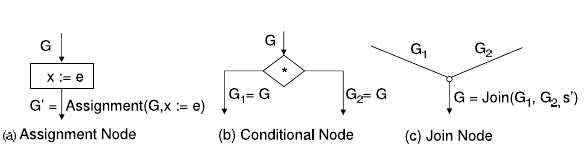
\includegraphics[scale=0.75]{GulwaniAlgorithm.png}}
    }
    \caption{Computation of SED for flowgraph nodes of a program}
    \label{fig:GulwaniAlgorithm}
\end{figure}

For detailed implementation of \texttt{Join} and \texttt{Assignment} 
functions, as well as a correctness proof of the algorithm, see 
\cite{Gulwani}.

\subsection{Complexity of the Algorithm}
\label{subsec:ComplexityOfTheAlgorithm}
The complexity of the algorithm is $\mathcal{O}(k^{3} * N * j)$, where 
$k$ is the total number of program variables, $N$ is the size of the 
program and $j$ is the number of join operations in the program. $k$ and 
$j$ are bounded by $N$, making the whole algorithm polynomial in $N$.

\section{Algorithm by Saleena and Paleri}
\label{sec:AlgorithmBySaleenAndPaleri}
Saleena and Paleri \cite{Saleena} gave an algorithm for \textbf{global 
value numbering (GVN)}. GVN works by assigning a \textbf{value number} 
to variables and expressions. The same value number is assigned to those 
variables and expressions which are provably equivalent. A notable 
difference between Herbrand equivalence and GVN is that in Herbrand 
equivalence one talks about equivalences at a particular program point 
but GVN is concerned with equivalence between expressions at two 
different program points.

The data structure used in the algorithm is called \textbf{value 
expression} - an expression with value numbers as operands. Two 
expressions are equivalent if they have same value expression. 
So, a value expression can be used to represent a set of equivalent 
program expressions.

\subsection{Notations}
\label{subsec:NotationsSaleena}
Input to the algorithm is a \textbf{flow graph} with atmost one assignment 
statement in each node which has one of the following forms
\begin{itemize} \tightlist
    \item $x\; ::=\; e$
    \item $e\ ::=\ x\ \mid\ c\ \mid\ x_1\ op\ x_2$
\end{itemize}
The flow graph also has two additional empty \texttt{ENTRY} and \texttt{EXIT} 
nodes. For a node $n$, \texttt{IN$_n$} and \texttt{OUT$_n$} denotes the input 
and output program points of the node.

\textbf{Expression pool} at a program point, is a partition of expressions 
at that point, in which equivalent expression belongs to the same partition. 
Each class will have a \textbf{value number} which will be considered as its 
first element. For a node $n$, \texttt{EIN$_n$} and \texttt{EOUT$_n$} denotes 
the expression pools at input and output program points of the node.

\subsection{Value Expression}
\label{subsec:ValueExpression}
The \textbf{value expression} corresponding to an expression is obtained 
by replacing the actual operands with their corresponding value numbers.
Example - For the expression pool $\{\{v_1, a, x\}$, $\{v_2, b, y \}\}$ 
and statement $z ::= x + y$ , the value expression for $x + y$ will be
$v_1 + v_2$. Instead of $x + y$, its value expression is included in 
the expression pool, with a new value number. So the new expression pool 
would be $\{\{v_1, a, x\},\{v_2, b, y\}, \{v_3, v_1 + v_2, z\}\}$.

The value expression $v_1 + v_2$ represents not just $x + y$ but the
set of equivalent expressions $\{a + b, x + b, a + y, x + y\}$. Its 
presence indicates that an expression from this set is already 
computed and this information is enough for detection of redundant 
computations. Also, a single binary value expression can represent 
equivalence among any numbre of expressions of any length. Example - 
$v_1 + v_3$ represents, $a + z$, $x + z$, $a + (a + b)$, 
$a + (x + b)$ and so on.

\subsection{Overview of the Algorithm}
\label{subsec:OverviewOfTheAlgorithmSaleena}
Similar to Gulwani's algorithm, the algorithm consists of two main 
functions - a \textbf{transfer} function for changes in expression pool 
across assignment statements and a \textbf{confluence function} to find 
the expression pool at points were two branches meet. The algorithm 
starts with \texttt{EOUT$_{\texttt{ENTRY}}$ = $\phi$}, and uses transfer 
and confluence functions to calculate expression pools at other points. 
This process is repeated till there is any change in the equivalence 
information. For detailed algorithm refer to \cite{Saleena}.

\section{Algorithm by Babu, Krishnan and Paleri}
\label{sec:AlgorithmByBabuKrishnanAndPaleri}
One problem is that most of these alogrithms are based on fix point 
computations but the classical definition of Herbrand equivalence is 
not a fix point based definition making it difficult to prove their 
precision or completeness. Babu, Krishnan and Paleri \cite{Babu} 
developed a lattice theoretic fix-point formulation of Herbrand 
equivalence on the lattice defined over the set of all terms constructible 
from variables, constants and operators of a program and showed that 
this definition is equivalent to the classical meet over all path 
characterization over the set of all possible expressions. They also 
proposed an algorithm which is able to detect all the equivalences as 
by that of Saleena and Paleri. This is discussed in detail in 
\autoref{chap:chapter3}.

\section{Conclusion}
\label{sec:Conclusion}
So to sum up, Kildall’s algorithm finds all the equivalent classes but 
is exponential. The algorithms by Saleena and Paleri; Babu, Krishnan 
and Paleri are polynomial and efficient among other imprecise algorithms. 
They are able to find all equivalence classes restricted to program 
expressions (all expressions with length atmost 2), which is precisely 
what is practically useful.
